\chapter{Desenvolvimento}\label{cap2}
 Nessa seção será apresentado o escopo do projeto e a proposta de solução.
\section{Escopo}
Para definição do escopo do projeto foram analisados os seguintes aspectos: local de atuação, situações de socorro pré-hospitalar, viabilidade dos itens a serem levados pelo VANT, elementos estruturais e planejamento e estratégia de voo do VANT e comunicação com o usuário.

\begin{description}
  \item[Local de Atuação] \hfill 
  	\begin{itemize}
  		\item Locais de difícil acesso no DF seja por natureza ou circunstância.
  	\end{itemize}
  \item[Tipo de emergência] \hfill 
  	\begin{itemize}
  		\item Parada Cardíaca
		\item Parada Respiratória
		\item Hemorragia Externa
  	\end{itemize}
  \item[Equipamentos Utilizados para salvamento] \hfill \\
  	Para definir os itens a serem levados foi realizada uma análise de viabilidade levando em consideração a utilização dos equipamentos por pessoas sem conhecimento em salvamento e a possibilidade de carga útil do VANT.
  	\begin{itemize}
  		\item Kit primeiro socorros
		\item Desfibrilador Automático
		\item Reanimador ventilatório manual
		\item Kit de hemorragias externas
  	\end{itemize}
  \item[Distância de Operação] \hfill 
  	\begin{itemize}
  		\item Haverá uma única central de controle
  		\item Velocidade máxima do drone: 70 km/h
  		\item O VANT operará em um raio de 80km. Sendo o centro do raio a ambulância onde se encontra o drone.
  	\end{itemize}
  \item[Sinais vitais que serão monitorados] \hfill 
  	\begin{itemize}
  		\item Eletrocardiograma
  	\end{itemize}
  \item[Projeto mecânico estrutural] \hfill 
  	\begin{itemize}
  		\item Asa rotatória
		\item Elétrico
  	\end{itemize}
  \item[Materiais] \hfill 
  	\begin{itemize}
  		\item Polímeros compostos
		\item Fibra de carbono
  	\end{itemize}
  \item[Controle] \hfill 
  	\begin{itemize}
  		\item Controle automático comandado pela central de comunicação. (Rádio frequência)
  	\end{itemize}
  \item[Comunicação entre equipe de paramédicos e usuário] \hfill 
  	\begin{itemize}
  		\item Câmera e sistema de áudio. Sendo que, o video será apenas para o paramédico da central e a comunicação via áudio para ambos.
  		\item O usuário apenas escutará as instruções, se comunicando apenas através do áudio.
  	\end{itemize}
  \item[Sensores] \hfill 
  	\begin{itemize}
  		\item Eletrocardiograma para medir os sinais vitais
		\item GPS - Utilizado para o deslocamento e localização do VANT
		\item Acelerômetro - Utilizado para obter uma localização mais apurada
		\item Giroscópio - Refinamento na localização
		\item Controlador A2 DJI
  	\end{itemize}
  \item[Projeto unidade central de processamento] \hfill 
  	\begin{itemize}
  		\item Controlador A2 DJI
  	\end{itemize}
  \item[Conversão e armazenamento de energia] \hfill 
  	\begin{itemize}
  		\item Bateria
  	\end{itemize}
  \item[Estimação de consumo energético e autonomia] \hfill 
  	\begin{itemize}
  		\item 4 horas de voo
  	\end{itemize}
\end{description}

\section{Estrutura Analítica de Projeto - EAP}

No desenvolvimento de qualquer projeto, é essencial ter uma visão geral sobre as atividades que serão realizadas no decorrer da processo de criação.  Para isso existem formas de sistematização e organização dessas informações.

Uma dessas formas de organizar a informação é a EAP - Estrutra Analítica do Projeto - que é a estruturação das entregas a serem completadas em forma de árvore de maneira hierárquica, onde são distribuídas da mais gerais para as mais especificas.

A EAP foi a forma escolhida pela equipe de desenvolvimento do projeto EmerVant para estruturação das entregas, por proporcionar de uma maneira simples e objetiva todos os pontos abordados e discutidos para a realização do projeto em seu devidos graus de importância. 

Para a criação da EAP do EmerVant, foi observado que dentro do projeto há varias áreas de atuação. Assim os níveis mais gerais foram definidos por essas áreas de atuação que são:
\begin{itemize}
\item Gerência de Projetos
\item Iniciação
\item Estrutura do VANT
\item Comunicação
\item Controle
\item Fonte Energética
\item Encerramento
\end{itemize}

\begin{figure}[ht]
  \centering
    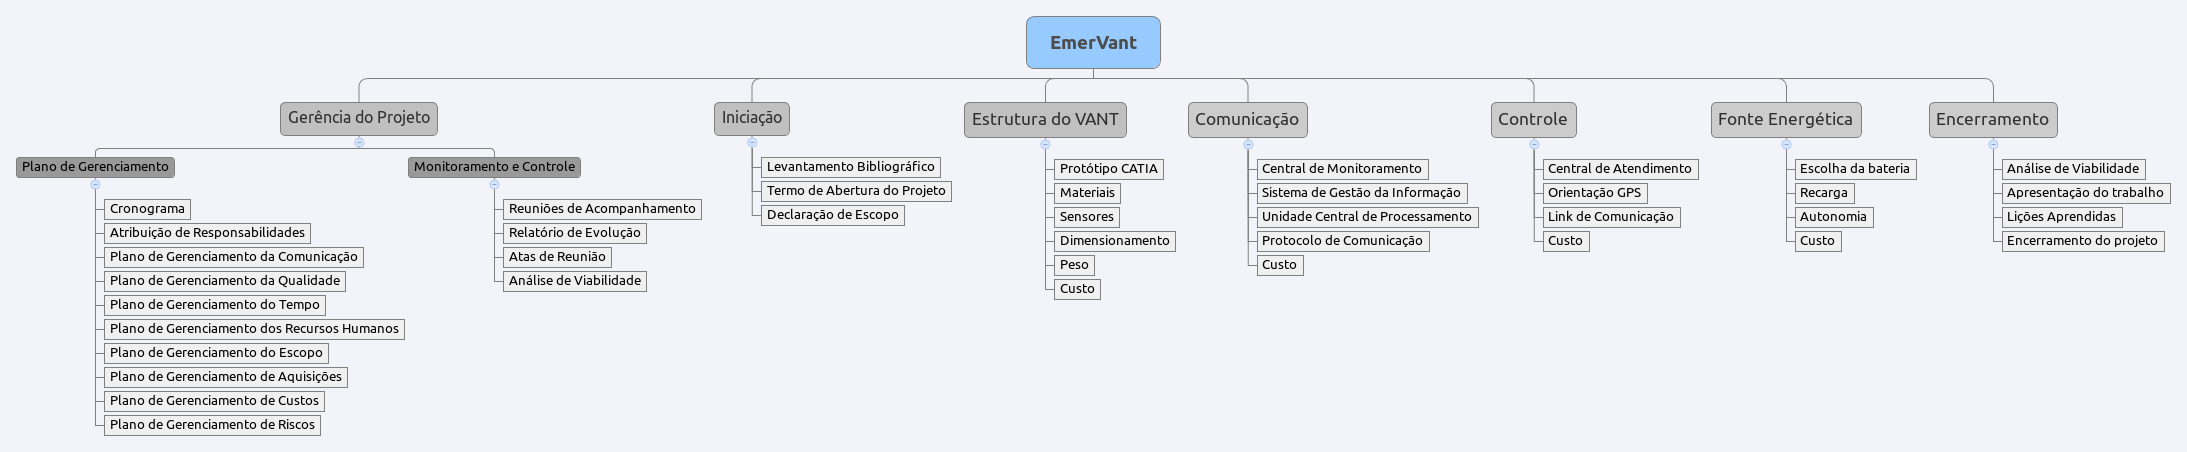
\includegraphics[keepaspectratio=true,scale=0.7,angle=90]{figuras/eap.eps}
  \caption{Estrutura Analítica do Projeto EmerVant}
\end{figure}

As entregas especificas de cada tópico foram baseadas nas definições de escopo e requisitos. A Figura 5 é a representação gráfica da EAP criada para o projeto EmerVant.

\section{Solução Inicial}
O EmerVant consiste em um sistema de assistência emergencial através da utilização de um VANT.  

O grande potencial dos drones tem sido explorado em inúmeras implementações militares e civis. Entre as vários VANTs, estes de pequena escala são especialmente atraentes para o meio acadêmico, devido ao seu pequeno tamanho, as capacidades de voo único, excelente dirigibilidade e baixo custo.\cite{SDM}

Também é possível que essas informações podem ser recebidas de fontes remotas, como GPS de satélites. Em uma situação normal o desempenho do piloto automático excede a controlada por humanos, e mesmo em situações mais desafiadoras sua performance é equivalente.

O projeto mecânico estrutural será constituído de polímeros compostos e fibra de carbono. O VANT será de asa rotatória e utilizará sistemas embarcados e sensores. O controle será feito através de um sistema automático com o uso de \textit{Global Position System} (GPS), utilizado para deslocamento e localização. 

O piloto automático deve ter acesso às informações em tempo real, e com isso computar a sua altitude, lugar no espaço e sua localização à obstáculos. Para gerar essas informações são necessários: giroscópios, acelerômetro, sensores magnéticos e eletromagnéticos, sensores visuais, infravermelhos, micro-ondas e gamas de rádio.\cite{UDE}

A partir isso, o tempo de voo foi estimado em quatro horas e o deslocamento do drone será com velocidade média de 70km/h e com raio de atuação de 80km da ambulância onde o mesmo está, a priori, acoplado. 

Esse sistema será monitorado através de uma central que receberá as informações referentes ao local e situação da(s) vítima(s) para repassá-las a ambulância e enviar as coordenadas para o VANT, que somente será ativado através da requisição da ambulância. 

O monitoramento do VANT ocorrerá através de um sistema de controle automático por rádio frequência que terá uma câmera e um sistema de áudio. 

O VANT através da câmera e do sistema de áudio estabelecerá a comunicação entre o usuário, a ambulância e a central de monitoramento. O vídeo será apresentado apenas para o paramédico da central e o áudio para a central e a ambulância. O contato do usuário será apenas com o áudio.

\section{Cronograma}
O cronograma preliminar das atividades pode ser visto na Figura 6, e o gráfico de Gantt que relaciona as tarefas com o tempo está representado na Figura 7. As atividades estão mais especificadas apenas no Ponto de Controle 1, os demais pontos de controle estão planejados de forma macro.

 \begin{figure}[ht]
	\centering
		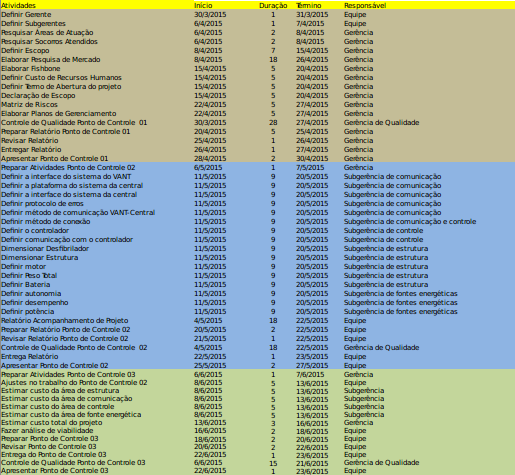
\includegraphics[keepaspectratio=true,scale=0.9]{figuras/cronograma.eps}
	\caption{Cronograma de Atividades}
\end{figure}

 \begin{figure}[ht]
	\centering
		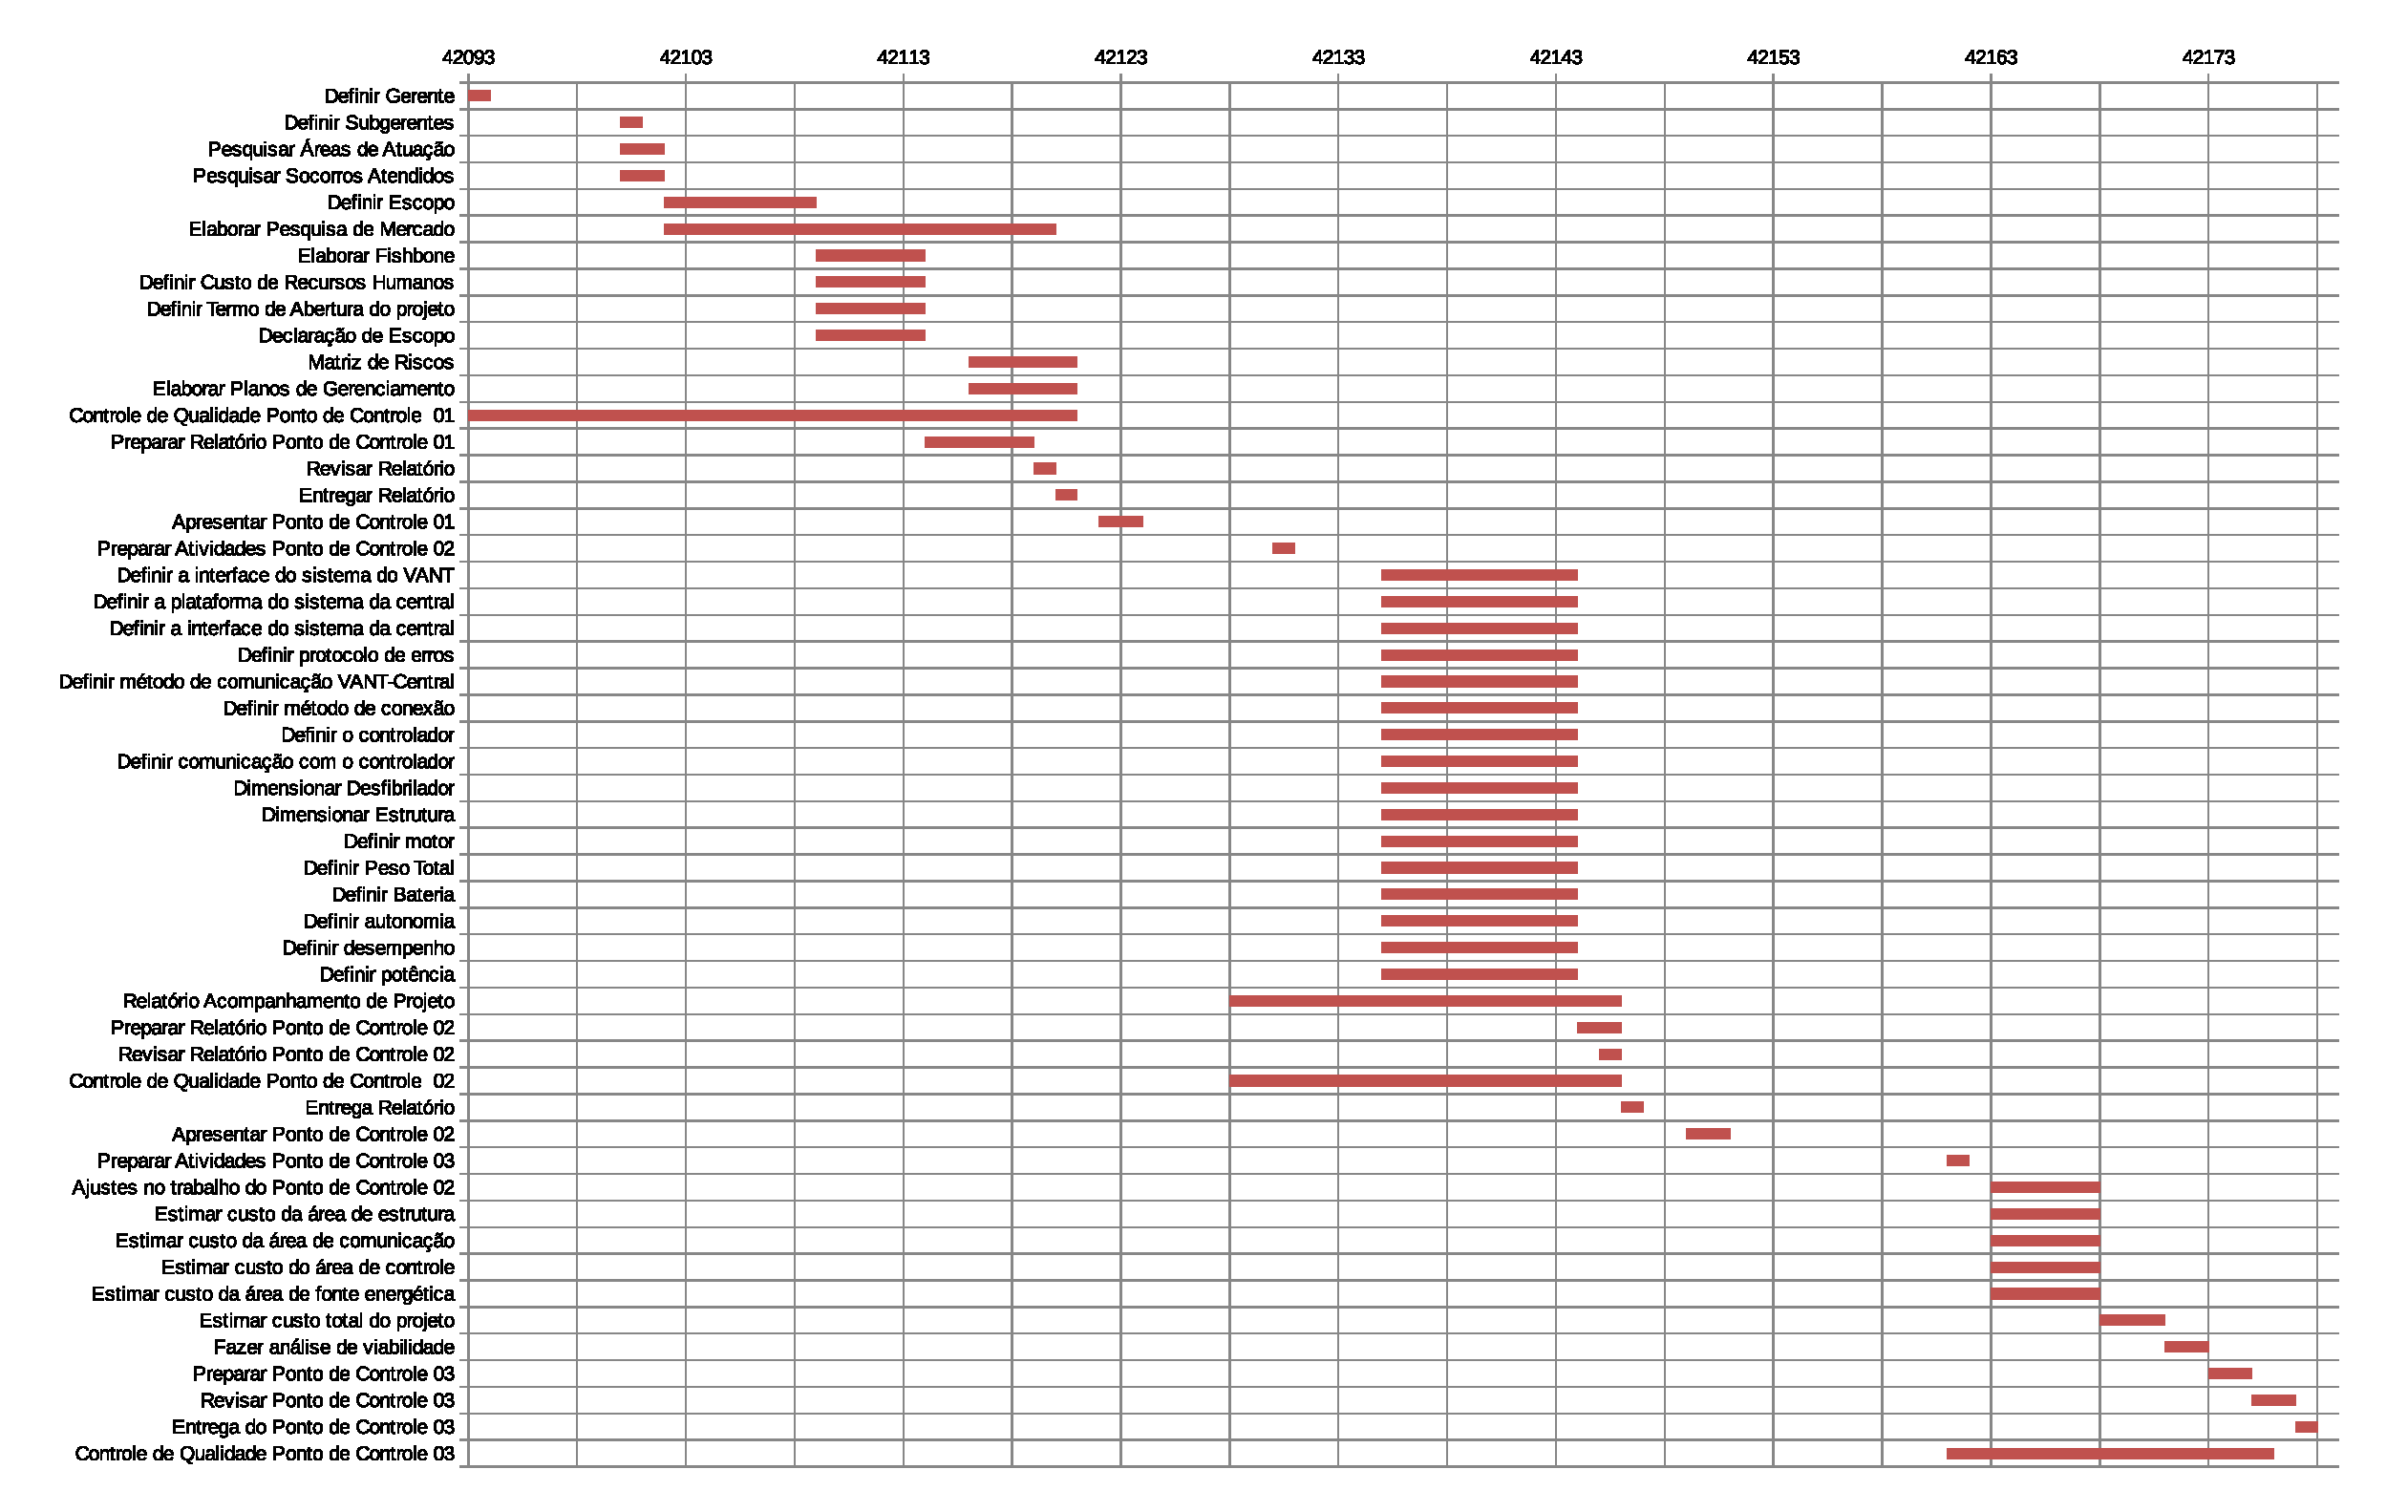
\includegraphics[keepaspectratio=true,scale=0.9,angle=90]{figuras/gantt.eps}
	\caption{Gráfico de Gantt}
\end{figure}


